\chapter{Φυσικοί αριθμοί}

\section{Οι αριθμοί και η Python}

Οι φυσικοί αριθμοί είναι οι αριθμοί από 0, 1, 2, 3, 4, 5, 6, \ldots, 98, 99, 100, \ldots, 1999, 2000, 2001, \ldots

Η Python μπορεί να χειριστεί φυσικούς αριθμούς. Δοκιμάστε να γράψετε στο REPL έναν φυσικό αριθμό, θα δείτε ότι η Python θα τον επαναλάβει. Π.χ. δείτε τον αριθμό εκατόν είκοσι τρια (123).
\begin{lstlisting}
>>> 123
123
\end{lstlisting}

Στην Python όμως θα πρέπει να ακολουθείς κάποιους επιπλέον κανόνες. Για παράδειγμα στους αριθμούς δεν πρέπει να βάζεις τελείες στις χιλιάδες όπως στο χαρτί. Αν το κάνεις στην καλύτερη περίπτωση θα προκύψει κάποιο λάθος, στην χειρότερη ο υπολογιστής θα καταλάβει διαφορετικό αριθμό από αυτόν που εννοείς.
Δείτε το παρακάτω παράδειγμα στο REPL.
\begin{lstlisting}
>>> 1.000.000
  File "<stdin>", line 1
    1.000.000
            ^
SyntaxError: invalid syntax
>>> 100.000
100.0
\end{lstlisting}
Σε αυτό το παράδειγμα, η Python δεν καταλαβαίνει καθόλου τον αριθμό 1.000.000 γραμμένο με τελείες ενώ μεταφράζει το 100.000 σε 100.0, που για την Python σημαίνει 100 (εκατό). Γι' αυτόν τον λόγο δεν βάζουμε καθόλου τελείες έτσι αν θέλουμε να γράψουμε το ένα εκατομμύριο θα γράψουμε 1000000.
\begin{lstlisting}
>>> 1000000
1000000
\end{lstlisting}

\section{Πρόσθεση, αφαίρεση και πολλαπλασιασμός φυσικών αριθμών}
Μια γλώσσα προγραμματισμού μπορεί να εκτελέσει απλές πράξεις πολύ εύκολα. Στο βιβλίο των μαθηματικών  σου μπορείς να βρεις πολλές ασκήσεις με πράξεις. Μπορείς να τις λύσεις με την Python.

\begin{exercise}
\sel{16}
Να υπολογιστούν τα γινόμενα: 

(α) $35 \cdot 10$, 

(β) $421 \cdot 100$,

(γ) $5 \cdot 1.000$,

(δ) $27 \cdot 10.000$
\end{exercise}

Η python μπορεί να κάνει αυτές τις πράξεις ως εξής:
\begin{lstlisting}
>>> 35*10
350
>>> 421*100
42100
>>> 5*1000
5000
>>> 27*10000
270000
\end{lstlisting}

Ο τελεστής του πολλαπλασιασμού είναι το αστεράκι * (SHIFT+8) στο πληκτρολόγιο. Εναλλακτικά, μπορείτε να το βρείτε στο αριθμητικό πληκτρολόγιο. 

\begin{exercise}
\sel{16}
Να εκτελεστούν οι ακόλουθες πράξεις:

(α) $89\cdot 7 + 89\cdot 3$

(β) $23 \cdot 49 + 77 \cdot 49$

(γ) $76 \cdot 13 – 76 \cdot 3$

(δ) $284 \cdot 99$
\end{exercise}
\begin{lstlisting}
>>> 89*7+89*3
890
>>> 23*49+77*49
4900
>>> 76*13-76*3
760
>>> 284*99
28116
\end{lstlisting}

Στις παραπάνω περιπτώσεις η python εκτελεί πρώτα τους πολλαπλασιασμούς και μετά τις προσθέσεις/αφαιρέσεις δίνοντας έτσι το αποτέλεσμα που αναμένεται. Για παράδειγμα 89\*7 + 89\*3 = 623 + 267 = 890, που είναι το σωστό αποτέλεσμα.

\begin{exercise}
\sel{18}
Υπολογίστε:

(α)  $157 + 33$ 

(β)  $122 + 25 + 78$

(γ)  $785 - 323$

(δ)  $7.321 - 4.595$

(ε)  $60 - (18 - 2)$

(στ) $52 - 11 -9$

(ζ)  $23 \cdot 10$

(η)  $97 \cdot 100$

(θ)  $879 \cdot 1.000$
\end{exercise}
Σε python τα παραπάνω υπολογίζονται ως εξής:
\begin{lstlisting}
>>> 157+33
190
>>> 122+25+78
225
>>> 785-323
462
>>> 7321-4595
2726
>>> 60-(18-2)
44
>>> 52-11-9
32
>>> 23*10
230
>>> 97*100
9700
>>> 879*1000
879000
\end{lstlisting}
Οι παρενθέσεις (SHIFT+9 και SHIFT+0) αλλάζουν τη σειρά των πράξεων. Οι πράξεις που είναι μέσα στην παρένθεση εκτελούνται πρώτες. Γι' αυτό το λόγο 60-(18-2)=60-16=44.

\begin{exercise}
\sel{18}
Σε ένα αρτοποιείο έφτιαξαν μία μέρα 120 κιλά άσπρο ψωμί, 135 κιλά χωριάτικο, 25 κιλά σικάλεως και 38 κιλά πολύσπορο. Πουλήθηκαν 107 κιλά άσπρο ψωμί, 112 κιλά χωριάτικο, 19 κιλά σικάλεως και 23 κιλά πολύσπορο. Πόσα κιλά ψωμί έμειναν απούλητα;
\end{exercise}
Με τις γνώσεις που έχουμε θα πρέπει να μετατρέψουμε το παραπάνω πρόβλημα σε μια αριθμητική παράσταση ώστε η python να μπορεί να την υπολογίσει, στη συγκεκριμένη περίπτωση η σωστή παράσταση είναι $$(120-107)+(135-112)+(25-19)+(38-23)$$
\begin{lstlisting}
>>> (120-107)+(135-112)+(25-19)+(38-23)
57
\end{lstlisting}
και η απάντηση είναι 57 κιλά ψωμί.

\section{Δυνάμεις φυσικών αριθμών}
Ο τελεστής της python για τις δυνάμεις είναι ο **  (δυο φορές το αστεράκι). Δηλαδή, αν θέλουμε να υπολογίσουμε το $10^2$ θα γράψουμε 10**2, με όμοιο τρόπο μπορούμε να υπολογίσουμε και τις υπόλοιπες δυνάμεις. Δοκίμασε τα παρακάτω στο REPL.
\begin{lstlisting}
>>> 10**2
100
>>> 10**3
1000
>>> 10**4
10000
>>> 10**5
100000
>>> 10**6
1000000
\end{lstlisting}
Στη προτεραιότητα των πράξεων, οι δυνάμεις έχουν μεγλύτερη προτεραιότητα από τον πολλαπλασιασμό και την πρόσθεση. Οπότε όταν έχουμε και δυνάμεις σε μια παράσταση πρώτα γίνονται οι πράξεις στις παρενθέσεις, μετά οι δυνάμεις και μετά οι πολλαπλασιασμοί και οι προσθέσεις. Την ίδια σειρά ακολουθεί και η python για τον υπολογισμό των πράξεων.
\begin{exercise}
\sel{21}
Να εκτελεστούν οι πράξεις 

 1. $(2\cdot 5)^4+4\cdot (3+2)^2$

 2. $(2+3)^3 - 8\cdot 3^2$

\end{exercise}
Οι αντίστοιχες εκφράσεις είναι (2*5)**4+4*(3+2)**2 και (2+3)**3 - 8*3**2.

\begin{lstlisting}
>>> (2*5)**4+4*(3+2)**2
10100
>>> (2+3)**3 - 8*3**2
53
\end{lstlisting}
H 8*3**2 υπολογίζεται ως $8\cdot (3^2)$, δηλαδή $8\cdot 9 = 72$, αφού πρώτα γίνεται η δύναμη και μετά οι πολλαπλασιασμοί.

\begin{exercise}
Κάνε τις πράξεις: 
(α) $3\cdot 5^2$, 

(β) $3\cdot 5^2 + 2$, 

(γ) $3\cdot5^2 + 2^2$, 

(δ) $3\cdot 5 + 2^2$, 

(ε) $3\cdot(5 + 2)^2$.
\end{exercise}

Αυτές οι πράξεις μπορούν να γίνουν στο REPL.
\begin{lstlisting}
>>> 3*5**2
75
>>> 3*5**2 + 2
77
>>> 3*5**2 + 2**2
79
>>> 3*5 +2**2
19
>>> 3*(5 + 2)**2
147
\end{lstlisting}

\begin{exercise}
Κάνε τις πράξεις: 
(α) $3^2 +3^3 +2^3 +2^4$, 

(β) $(13-2)^ 4 + 5\cdot 3^2$
\end{exercise}

\begin{lstlisting}
>>> 3**2 +3**3 +2**3 +2**4
60
>>> (13-2)**4 + 5*3**2
14686
\end{lstlisting}

\begin{exercise}
Βρες τις τιμές των παραστάσεων: 

(α) $(6+5)^2$ και $6^2+5^2$, 

(β) $(3+6)^2$ και $3^2+6^2$.
\end{exercise}
\begin{lstlisting}
>>> (6+5)**2
121
>>> 6**2+5**2
61
>>> (3+6)**2
81
>>> 3**2+6**2
45
\end{lstlisting}


\section{Συγκρίσεις φυσικών αριθμών}
Μπορούμε να συγκρίνουμε αριθμούς στην Python χρησιμοποιώντας τους τελεστές == (πληκτρολογούμε δύο φορές το =) για την \emph{ισότητα}, > για το \emph{μεγαλύτερο} και < για το \emph{μικρότερο}. Επίσης μπορούμε να χρησιμοποιήσουμε >= για το \emph{μεγαλύτερο ή ίσο} και <= για το \emph{μικρότερο ή ίσο}, τέλος υπάρχει το != για το \emph{δεν είναι ίσο}. Μπορείς να δοκιμάσεις τα παρακάτω:
\begin{lstlisting}
>>> 123==123
True
>>> 123>123
False
>>> 123>122
True
>>> 123<123
False
>>> 123<124
True
>>> 123<=123
True
>>> 123<=124
True
>>> 123<=122
False
>>> 123>=123
True
>>> 123>=124
False
>>> 123>=122
True
>>> 122 != 123
True
>>> 122 != 122
False
\end{lstlisting}
Η Python επιστρέφει True (αληθές) όταν μία πρόταση ισχύει και False (ψευδές) όταν δεν ισχύει.

Σκέψου ότι για την Python η σύγκριση είναι και αυτή μια πράξη. Αντί η πράξη αυτή να δίνει σαν αποτέλεσμα έναν αριθμό δίνει σαν αποτέλεσμα το αληθές ή το ψευδές.

Για παράδειγμα:
\begin{exercise}
Να συγκρίνετε τα $3^2$ και $2^3$.
\end{exercise}
Η σύγκριση αυτή μπορεί να γίνει στο REPL. Δοκίμασε:
\begin{lstlisting}
>>> 3**2 > 2**3
True
\end{lstlisting}
Άρα το $3^2$ είναι μεγαλύτερο από το $2^3$. Θυμήσου ότι το $3^2=9$, ενώ $2^3=8$.
\begin{exercise}
\end{exercise}

\section{Η εντολή print}
Ήρθε η ώρα να γράψεις εντολές στο πάνω παράθυρο, δηλαδή να γράψεις το πρώτο σου πρόγραμμα.  Με βάση όσα ξέρεις προσπάθησε να γράψεις μια πράξη στο πάνω παράθυρο, για παράδειγμα $32+35$. Ύστερα πάτησε το κουμπί της εκτέλεσης (Run). Μπορείς να δεις το αποτέλεσμα στην εικόνα \ref{noprint}.
\begin{figure}
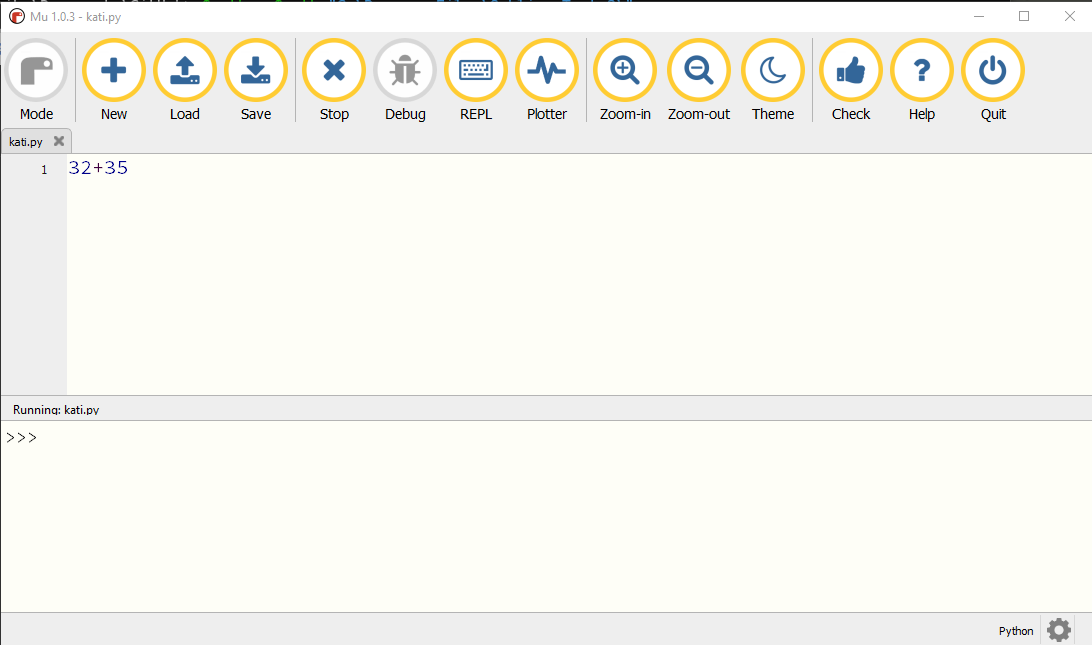
\includegraphics[width=\textwidth]{noprint.png}
\caption{Η εκτέλεση δεν δίνει κάποιο αποτέλεσμα}
\label{noprint}
\end{figure}

Η Python εκτελεί την πράξη $32+35$, και υπολογίζει το αποτέλεσμα. Αν δεν το έκανε και υπήρχε κάποιο πρόβλημα θα εμφάνιζε κάποιο μήνυμα λάθους στο REPL. Το υπολογισμένο αποτέλεσμα δεν εμφανίζεται. Για να εμφανιστεί το αποτέλεσμα πρέπει να χρησιμοποιήσεις την εντολή print (εκτύπωσε). Η εντολή print εκτελείται ως εξής:
\begin{lstlisting}
print(32+35)
\end{lstlisting}
Γράφουμε δηλαδή, print ανοίγουμε παρένθεση, γράφουμε αυτό που θέλουμε να εκτυπωθεί και κλείνουμε την παρένθεση. Όταν εκτελέσουμε το πρόγραμμα με την print τότε εμφανίζεται το αποτέλεσμα στο REPL (εικόνα \ref{withprint}).
\begin{figure}
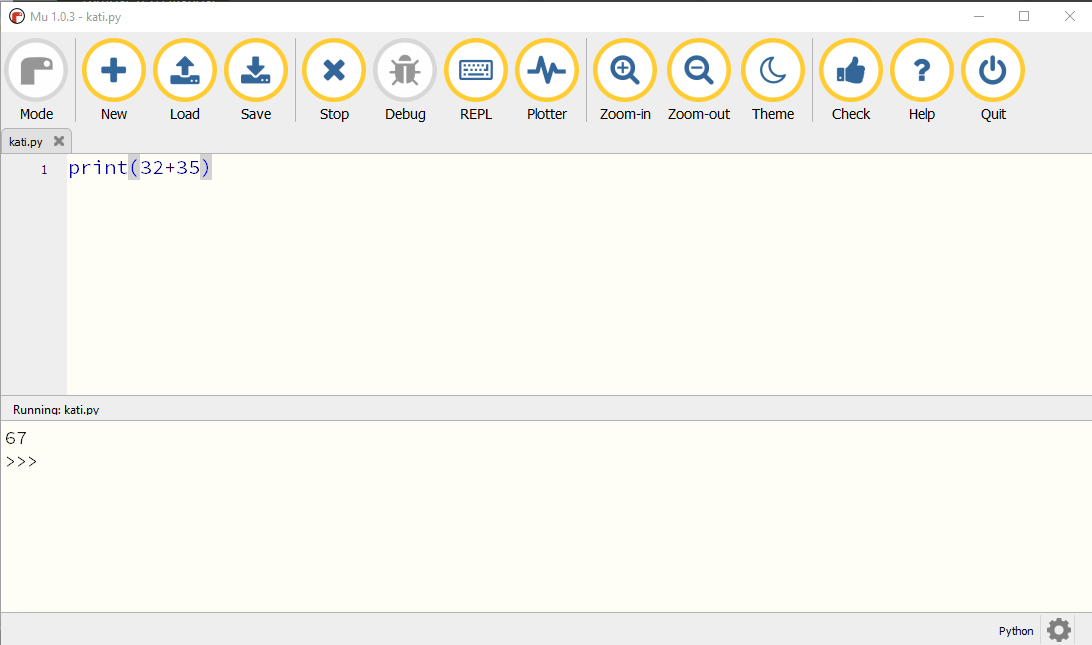
\includegraphics[width=\textwidth]{withprint.png}
\caption{Η εκτέλεση δίνει το αποτέλεσμα της πράξης}
\label{withprint}
\end{figure}
Μόλις έγραψες το πρώτο σου πρόγραμμα στην Python. Μάλιστα το πρόγραμμά σου κάνει κάτι. Υπολογίζει το αποτέλεσμα της πράξης $32+35$.
Μπορείς να αποθηκεύσεις το πρόγραμμά σου στον υπολογιστή σου κάνοντας κλικ στο εικονίδιο Save του Mu (εικόνα \ref{savewithmu}).
\begin{figure}
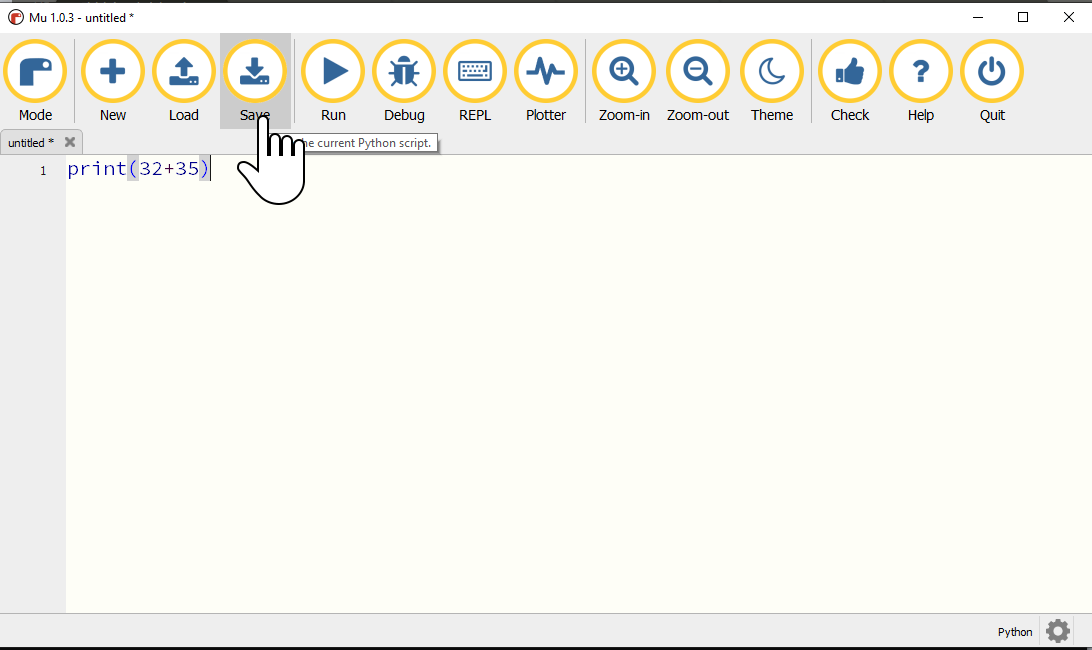
\includegraphics[width=\textwidth]{save.png}
\caption{Αποθήκευση με το Mu}
\label{savewithmu}
\end{figure}

\section{Απαρίθμηση}
Είδαμε ότι η Python μπορεί να κάνει πολύ γρήγορα, πολύπλοκες πράξεις ακόμη και με δυνάμεις, αλλά δεν είδαμε ακόμη τις απλές ασκήσεις που υπάρχουν στις πρώτες σελίδες του βιβλίου. Όπως για παράδειγμα ποιοι είναι οι τρεις προηγούμενοι αριθμοί του 289 και ποιο οι δύο επόμενοι \sel{13}.

Τώρα που μάθαμε να γράφουμε προγράμματα σε Python μπορούμε να αντιμετωπίσουμε αυτό το πρόβλημα με το παρακάτω πρόγραμμα:
\begin{lstlisting}
print(289-3)
print(289-2)
print(289-1)
print(289+1)
print(289+2)
\end{lstlisting}
που δίνει το αποτέλεσμα
\begin{lstlisting}
286
287
288
290
291
\end{lstlisting}

Πιο σωστό θα ήταν να γράψουμε ποιοι αριθμοί είναι οι προηγούμενοι και ποιοι οι επόμενοι. Σε αυτή την περίπτωση θα γράψουμε τις παρακάτω εντολές.
\begin{lstlisting}
print("Οι  προηγούμενοι αριθμοί είναι:")
print(289-3)
print(289-2)
print(289-1)
print("Οι επόμενοι αριθμοί είναι:")
print(289+1)
print(289+2)
\end{lstlisting}

Για να εμφανίσει η print τις λέξεις που θέλουμε πρέπει να τις βάλουμε μέσα σε εισαγωγικά. Η Python υποστηρίζει είτε μονά εισαγωγικά, είτε διπλά. Αυτά εισάγονται συνήθως με το ίδιο κουμπί του πληκτρολογίου (κοντά στο ENTER), είτε με SHIFT ή χωρίς. Θυμήσου να κλείνεις τα εισαγωγικά με τον ίδιο τρόπο που τα άνοιξες. Στο πρόγραμμα Mu τα εισαγωγικά αυτά δεν φαίνονται όπως σε άλλα πρόγραμματα σαν `Εισαγωγικά' ή ``Εισαγωγικά " ή <<Εισαγωγικά>>, αλλά φαίνονται κάπως πιο απλά και ίδια στο άνοιγμα και το κλείσιμο \lstinline{'Εισαγωγικά'} ή  \lstinline{"Εισαγωγικά"}. 

Αν θέλουμε να αλλάξουμε το 289 και να βάλουμε έναν άλλο αριθμό,π.χ. το 132 θα πρέπει να αντικαταστήσουμε το 289 μέσα σε όλες τις εντολές print με το 132.
\begin{lstlisting}
print("Οι προηγούμενοι αριθμοί είναι:")
print(132-3)
print(132-2)
print(132-1)
print("Οι επόμενοι αριθμοί είναι:")
print(132+1)
print(132+2)
\end{lstlisting}

Υπάρχει όμως ένας καλύτερος τρόπος, ο τρόπος αυτός είναι να δώσουμε ένα όνομα στον αριθμό μας. Μπορούμε να πούμε ότι το n είναι το όνομα του αριθμού. Αυτό γίνεται με την εντολή \lstinline{n=132}. Τότε το πρόγραμμά μας γίνεται:
\begin{lstlisting}
n = 132
print("Οι προηγούμενοι αριθμοί είναι:")
print(n-3)
print(n-2)
print(n-1)
print("Οι επόμενοι αριθμοί είναι:")
print(n+1)
print(n+2)
\end{lstlisting}

Μετά την εντολή \lstinline{n=132} η Python ξέρει ότι το n είναι ένα όνομα για το 132 και μπορεί να κάνει πράξεις με αυτό. Για παράδειγμα n+1 κάνει τώρα 133.

Αν θέλουμε να κάνουμε τώρα το ίδιο πρόγραμμα αλλά όχι για το 132 αλλά για το 210, χρειάζεται να αλλάξουμε μόνο μία γραμμή και το πρόγραμμά μας να γίνει ως εξής:
\begin{lstlisting}
n = 210
print("Οι προηγούμενοι αριθμοί είναι:")
print(n-3)
print(n-2)
print(n-1)
print("Οι επόμενοι αριθμοί είναι:")
print(n+1)
print(n+2)
\end{lstlisting}

Στην Python, όταν δίνουμε ένα όνομα σε έναν αριθμό (με τον τελεστή =) τότε δημιουργούμε μια μεταβλητή. Η μεταβλητή έχει ένα όνομα, στην περίπτωσή μας το n, και μια τιμή, στην περίπτωσή μας το 210.

Αν αντί για τους επόμενους δύο αριθμούς θέλαμε τους επόμενους \textbf{δέκα} θα γράφαμε ένα πρόγραμμα όπως το παρακάτω:
\begin{lstlisting}
n = 210
print(n)
print(n+1)
print(n+2)
print(n+3)
print(n+4)
print(n+5)
print(n+6)
print(n+7)
print(n+8)
print(n+9)
print(n+10)
\end{lstlisting}
Το παραπάνω πρόγραμμα εμφανίζει και τον αριθμό μας n, δηλαδή το 210.

Για να μην γράφουμε πολλές εντολές όταν κάνουμε το ίδιο πράγμα χρησιμοποιούμε την εντολή for.
Το πρόγραμμά μας με την for μπορεί να γίνει:
\begin{lstlisting}
n = 210
for i in 0,1,2,3,4,5,6,7,8,9,10:
    print(n+i)
\end{lstlisting}
Όταν γράψεις την for στην Python θα πρέπει να δηλώσεις ποιες εντολές θα εκτελεστούν πολλές φορές. Αυτή η δήλωση γίνεται βάζοντας αυτές τις εντολές λίγο πιο μέσα χρησιμοποιώντας το πλήκτρο κενό ή το πλήκτρο tab. Μια καλή πρακτική είναι να βάζεις τέσσερα κενά. Έτσι, πριν την εντολή \lstinline{print(n+i)} βάζεις τέσσερα κενά δηλαδή \lstinline[showspaces=true]{    print(n+i)}.
Το πρόγραμμα αυτό σημαίνει πως για το i μέσα στο σύνολο 0, 1, 2, 3, \ldots 10 και με αυτή τη σειρά εμφάνισε το n+i. Έτσι το αποτέλεσμα είναι το αναμενόμενο
\begin{lstlisting}
210
211
212
213
214
215
216
217
218
219
220
\end{lstlisting}

Στην Python υπάρχει ένας πιο εύκολος τρόπος να γράψουμε τους αριθμούς από το 0 έως το 10. Αυτός ο τρόπος είναι η εντολή range και συγκεκριμένα η range(11). Η range(11) φτιάχνει τους αριθμούς από το 0 μέχρι το 10 οι οποίοι είναι σε πλήθος 11. 
Έτσι το πρόγραμμά μας γίνεται:
\begin{lstlisting}
n = 210
for i in range(11):
    print(n+i)
\end{lstlisting}

Mπορούμε και να μετρήσουμε τους πρώτους 100 αριθμούς ως εξής:
\begin{lstlisting}
for i in range(100):
    print(i)
\end{lstlisting}

Σκέψου αν θα δεις τον αριθμό 100 στο αποτέλεσμα του παραπάνω προγράμματος.

Μπορούμε να δούμε αριθμούς εύκολα με την Python αλλά θα χρειαστεί ξεχωριστό πρόγραμμα αν θέλουμε να εμφανίζεται το λεκτικό  για κάθε αριθμό.

Ένα τέτοιο πρόγραμμα είναι το παρακάτω:
\begin{lstlisting}
print('μηδέν')
print('ένα')
print('δύο')
print('τρία')
print('τέσσερα')
print('πέντε')
print('έξι')
print('εφτά')
print('οχτώ')
print('εννιά')
print('δέκα')
print('έντεκα')
print('δώδεκα')
print('δεκατρία')
print('δεκατέσσερα')
print('δεκαπέντε')
print('δεκαέξι')
print('δεκαεφτά')
print('δεκαοχτώ')
print('δεκαεννιά')
\end{lstlisting}

Το παραπάνω πρόγραμμα μπορεί να γίνει πιο μαζεμένο με τη χρήση λίστας. Μια λίστα μπορεί να περιέχει τα λεκτικά για κάθε αριθμό. Η λίστα στην Python σημειώνεται με τις τετράγωνες αγκύλες \[ και \]. Τα στοιχεία της χωρίζονται με κόμμα. Έτσι η λίστα που θέλουμε τώρα είναι η εξής:
\begin{lstlisting}
lektika = ['μηδέν','ένα','δύο','τρία','τέσσερα','πέντε','έξι','εφτά','οχτώ','εννιά','δέκα','έντεκα','δώδεκα','δεκατρία','δεκατέσσερα','δεκαπέντε','δεκαέξι','δεκαεφτά','δεκαοχτώ','δεκαεννιά']
\end{lstlisting}
Χρησιμοποιούμε τις τετράγωνες αγκύλες και τον αριθμό του στοιχείου που θέλουμε να προσπελάσουμε σε μια λίστα. Η αρίθμηση της λίστας ξεκινάει από το 0. Έτσι, στη λίστα που βλέπουμε παραπάνω το lektika[0] θα είναι η λέξη 'μηδέν' (θυμηθείτε τα εισαγωγικά), το lektika[1] θα είναι η λέξη 'ένα' κ.ο.κ.

Αν θέλετε μπορείτε να κάνετε μια μικρή δοκιμή στο REPL.
\begin{lstlisting}
>>>lektika = ['μηδέν','ένα','δύο']
>>>lektika[0]
μηδέν
>>>lektika[1]
ένα
>>>lektika[2]
δύο
\end{lstlisting}
Με τη χρήση της λίστας μπορούμε να εμφανίσουμε τους αριθμούς με τη σειρά χρησιμοποιώντας την εντολή for.
\begin{lstlisting}
lektika = ['μηδέν','ένα','δύο','τρία','τέσσερα','πέντε','έξι','εφτά',
'οχτώ','εννιά','δέκα','έντεκα','δώδεκα','δεκατρία',
'δεκατέσσερα','δεκαπέντε','δεκαέξι','δεκαεφτά','δεκαοχτώ',
'δεκαεννιά']
for i in range(20):
    print(lektika[i])
\end{lstlisting}

Όμως παρότι δεν γράφουμε είκοσι φορές την εντολή print πάλι δίνουμε όλα τα ονόματα στο πρόγραμμά μας βάζοντάς τα σε μια λίστα. Μπορούμε να το αποφύγουμε υπολογίζοντας το λεκτικό. Από το δώδεκα και μέτα το λεκτικό ενός αριθμού i είναι το `δεκα' και μετά το λεκτικό του αριθμού i-10. Για παράδειγμα, το δεκαοχτώ είναι το `δεκα' ακολουθούμενο από το λεκτικό του αριθμού που προκύπτει αν αφαιρέσουμε 10 από το 18.

Η Python μπορεί να κάνει πράξεις και με τις λέξεις, η πρόσθεση λέξεων σημαίνει να τις βάλεις δίπλα δίπλα με τη σειρά. Δοκίμασε 
\begin{lstlisting}
In [1]: 'δεκα' + 'τρία'
Out[1]: 'δεκατρία'
\end{lstlisting}
Με αυτή την ευκολία το πρόγραμμά μας γίνεται:
\begin{lstlisting}
lektika = ['μηδέν','ένα','δύο','τρία','τέσσερα','πέντε','έξι','εφτά',
'οχτώ','εννιά','δέκα','έντεκα','δώδεκα','δεκατρία',
'δεκατέσσερα','δεκαπέντε','δεκαέξι','δεκαεφτά','δεκαοχτώ',
'δεκαεννιά']
for i in range(20):
    if i<=12:
        print(lektika[i])
    else:
        print('δεκα'+lektika[i-10])
\end{lstlisting}


Μάλιστα, το πρόγραμμα υπολογίζει τα λεκτικά από το 13 και μετά και δεν χρειάζεται να τα θυμάται. Μπορούμε να τα διαγράψουμε από τη λίστα.
\begin{lstlisting}
lektika = ['μηδέν','ένα','δύο','τρία','τέσσερα','πέντε','έξι','εφτά',
'οχτώ','εννιά','δέκα','έντεκα','δώδεκα']
for i in range(20):
    if i > 12:
        print('δέκα'+lektika[i-10])
    else:
        print(lektika[i])
\end{lstlisting}

Τώρα μπορούμε να πάμε μέχρι το 29.
\begin{lstlisting}
lektika = ['μηδέν','ένα','δύο','τρία','τέσσερα','πέντε','έξι','εφτά',
'οχτώ','εννιά','δέκα','έντεκα','δώδεκα']
for i in range(30):
    if i>20:
        print('είκοσι' + lektika[i-20])
    elif i > 12:
        print('δέκα'+lektika[i-10])
    else:
        print(lektika[i])
\end{lstlisting}
Το elif είναι συντομογραφία για το else if. Στο σημείο που το έβαλες τώρα σημαίνει αν το i δεν είναι μεγαλύτερο του 20 (else) και είναι μεγαλύτερο από το 12 (if). Άρα το \lstinline{print('δέκα'+lektika[i-10])} γίνεται μόνο αν το i είναι μικρότερο ή ίσο του 20 και μεγαλύτερο από 12.
Το αποτέλεσμα φαίνεται παρακάτω:
\begin{lstlisting}
 ένα  
 δύο 
 τρία 
 τέσσερα 
 πέντε 
 έξι 
 εφτά 
 οχτώ 
 εννιά 
 δέκα 
 έντεκα 
 δώδεκα 
 δέκατρία 
 δέκατέσσερα 
 δέκαπέντε 
 δέκαέξι 
 δέκαεφτά 
 δέκαοχτώ 
 δέκαεννιά 
  (*@\textcolor{blue}{δέκαδέκα}@*) 
 είκοσιένα 
 είκοσιδύο 
 είκοσιτρία 
 είκοσιτέσσερα 
 είκοσιπέντε 
 είκοσιέξι 
 είκοσιεφτά 
 είκοσιοχτώ 
 είκοσιεννιά 
\end{lstlisting}
Οπότε καταλαβαίνουμε ότι το είκοσι χρειάζεται ειδικό χειρισμό. Με τη χρήση της elif μπορούμε να βάλουμε και ειδικό χειρισμό για το 20.
\begin{lstlisting}
lektika = ['μηδέν','ένα','δύο','τρία','τέσσερα','πέντε','έξι','εφτά',
'οχτώ','εννιά','δέκα','έντεκα','δώδεκα']
for i in range(30):
    if i>20:
        print('είκοσι' + lektika[i-20])
    elif i==20:
        print('είκοσι')
    elif i > 12:
        print('δέκα'+lektika[i-10])
    else:
        print(lektika[i])
\end{lstlisting}
\begin{lstlisting}
 ένα  
 δύο 
 τρία 
  .
  .
  .
 έντεκα 
 δώδεκα 
 δέκατρία 
  .
  .
  .
 δέκαεννιά 
 (*@\textcolor{blue}{είκοσι}@*) 
 είκοσιένα
  .
  .
  .
 είκοσιεννιά 
\end{lstlisting}


\section{Στρογγυλοποίηση}
Το βιβλίο των Μαθηματικών της Α' Γυμνασίου αναφέρει πως
Για να στρογγυλοποιήσουμε έναν φυσικό αριθμό \sel{12}:
\begin{enumerate}
	\item Προσδιορίζουμε την τάξη στην οποία θα γίνει η στρογγυλοποίηση
	\item Εξετάζουμε το ψηφίο της αμέσως μικρότερης τάξης
	\item Αν αυτό το ψηφίο είναι μικρότερο του 5 (δηλαδή 0, 1, 2, 3 ή 4) το ψηφίο αυτό και όλα τα ψηφία των υπόλοιπων τάξεων μηδενίζονται.
	\item Αν είναι μεγαλύτερο ή ίσο του 5 (δηλαδή 5, 6, 7, 8 ή 9) το ψηφίο αυτό και όλα τα ψηφία των υπόλοιπων τάξεων αντικαθίστανται από το 0 και το ψηφίο της τάξης στρογγυλοποίησης αυξάνεται κατά 1.
\end{enumerate}

Ας πούμε ότι θέλουμε να στρογγυλοποιήσουμε τον αριθμό 454.018.512 στα εκατομμύρια. Η απάντηση που περιμένουμε είναι 454 εκατομμύρια.
Για να τα καταφέρουμε θα χρησιμοποιήσουμε την διαίρεση. Όμως στην Python υπάρχουν \emph{δύο} διαιρέσεις μία με το σύμβολο/και μία με το σύμβολο //. Ας δούμε τις διαφορές τους στο REPL.
\begin{lstlisting}
>>> x = 454018512
>>> print(x/1000000)
454.018512
>>> print(x//1000000)
454
\end{lstlisting}
Η <<κανονική>> διαίρεση, με τη μία κάθετο /, δίνει το αποτέλεσμα της διαίρεσης με τα δεκαδικά ψηφία. Η <<ακέραια>> διαίρεση δίνει μόνο τον ακέραιο αριθμό. Δεν μπορούμε να πούμε ότι η ακέραια διαίρεση θα μας δώσει την στρογγυλοποίηση γιατί η ακέραια διαίρεση δεν στρογγυλοποιεί τα δεκαδικά ψηφία αλλά τα απορρίπτει εντελώς. Έτσι, ακόμη και αν είχαμε 454918512 κατοίκους η ακέραια διαίρεση θα δώσει 454 αντί για το στρογγυλοποιημένο που είναι 455.
\begin{lstlisting}
>>> x = 454918512
>>> print(x/1000000)
454.918512
>>> print(x//1000000)
454
\end{lstlisting}

Χρειάζεται επομένως να δούμε το ψηφίο της αμέσως χαμηλότερης τάξης το οποίο είναι το πρώτο δεκαδικό της κανονικής διαίρεσης. Για να το απομονώσουμε αφαιρούμε από το αποτέλεσμα της κανονικής διαίρεσης το ακέραιο μέρος.
\begin{lstlisting}
>>> x = 454018512
>>> x/1000000 - x//1000000
0.018511999999986983
\end{lstlisting}
Οπότε τώρα έχουμε δύο ενδεχόμενα αν το αποτέλεσμα αυτής της πράξης είναι μικρότερο από 0.5 όπως παραπάνω τότε το αποτέλεσμα που ψάχνουμε είναι το αποτέλεσμα της ακέραιας διαίρεσης. Αλλιώς πρέπει να προσθέσουμε ένα στο αποτέλεσμα της ακέραιας διαίρεσης.
Αυτό γίνεται με την εντολή if, που σημαίνει στα αγγλικά αν. Για ευκολία μπορούμε να ονομάσουμε d την διαφορά των δύο διαιρέσεων με την εντολή:
\begin{lstlisting}
d = x/1000000 - x//1000000
\end{lstlisting}
Επειδή το πρόγραμμα γίνεται μεγαλύτερο τώρα θα το γράψουμε στο πάνω παράθυρο του Mu.
\begin{lstlisting}
x = 454018512
d = x/1000000 - x//1000000
if d < 0.5:
    print(x//1000000)
else:
    print(x//1000000 + 1)
\end{lstlisting}
Την \lstinline{if} την γράφουμε ως εξής:
\begin{lstlisting}
if συνθήκη:
    εντολές που εκτελούνται
    αν ισχύει η συνθήκη
else:
    εντολές που εκτελούνται
    αν δεν ισχύει η συνθήκη
\end{lstlisting}
Θυμήσου να βάζεις την άνω κάτω τελεία μετά τη συνθήκη και μετά τη λέξη else που σημαίνει αλλιώς.

Αν στο ίδιο πρόγραμμα και βάλεις αντί για 454.018.512 τον αριθμό 454.918.512 θα δεις ότι θα εμφανιστεί το σωστό αποτέλεσμα (455).

Αν θέλεις στρογγυλοποίηση στις χιλιάδες τότε το πρόγραμμά σου γίνεται:
\begin{lstlisting}
x = 454018512
d = x/1000 - x//1000
if d < 0.5:
    print(x//1000)
else:
    print(x//1000 + 1)
\end{lstlisting}
και το αποτέλεσμα είναι 454019.

\begin{exercise}
Για να γίνει το 454.018.512, 450 εκατομμύρια \sel{12} η στρογγυλοποίηση γίνεται στις δεκάδες των εκατομμυρίων. Μπορείς να γράψεις ένα πρόγραμμα που να στρογγυλοποιεί αριθμούς στις δεκάδες των εκατομμυρίων;
\end{exercise}

\section{Επανάληψη στις πράξεις}
\begin{exercise}
Συμπλήρωσε τον πίνακα τα τετράγωνα και τους κύβους των αριθμών από το 8 μέχρι το 25 \sel{22}.
\end{exercise}
\begin{lstlisting}
for a in range(8,26):
    print(a**2,end =" ")
print()
print()
for a in range(8,26):
    print(a**3,end=" ")
\end{lstlisting}
Το αποτέλεσμα αυτού του προγράμματος είναι:

\begin{lstlisting}
64 81 100 121 144 169 196 225 256 289 324 361 400 441 484 529 576 625 

512 729 1000 1331 1728 2197 2744 3375 4096 4913 5832 6859 8000 9261 
10648 12167 13824 15625
\end{lstlisting}

Η εντολή print μπορεί να πάρει περισσότερα από ένα ορίσματα, το πρώτο όρισμα είναι αυτό που θα εμφανίσει. Το δεύτερο όρισμα που δώσαμε είναι το end και το ορίσαμε ίσο με το κενό (\lstinline{end=" "}) που σημαίνει ότι η print όταν εμφανίσει το πρώτο όρισμα δεν θα αλλάξει γραμμή αλλά θα αφήσει ένα κενό. Η εντολή print() αλλάζει απλά γραμμή.
\begin{exercise}
Βρες τα τετράγωνα των αριθμών 10,20,30,40,50,60,70,80 και 90 \sel{22}.
\end{exercise}
Το πρόγραμμα είναι το εξής:
\begin{lstlisting}
for i in range(10,100,10):
    print(i**2,end=',')
\end{lstlisting}
και το αποτέλεσμα της εκτέλεσης του προγράμματος είναι
\begin{lstlisting}
100,400,900,1600,2500,3600,4900,6400,8100,
\end{lstlisting}

\begin{exercise}
Βρες τους κύβους των αριθμών 10,20,30,40,50
\end{exercise}

\begin{lstlisting}
for i in range(10,60,10):
    print(i**3,end=', ')  
\end{lstlisting}
Το αποτέλεσμα της εκτέλεσης είναι:
\begin{lstlisting}
1000, 8000, 27000, 64000, 125000, 
\end{lstlisting}

\section{Ανάπτυγμα}
\begin{exercise}\sel{21}Να γραφεί το ανάπτυγμα του αριθμόύ 7.604 με χρήση των δυνάμεων του 10.
\end{exercise}
Η απάντηση είναι $7\cdot 10^3 + 6\cdot 10^2 + 0\cdot 10^1 + 4$.  Με συμβολισμό της Python η απάντηση που περιμένουμε είναι:
\begin{lstlisting}
7*10**3+6*10**2+0*10+4
\end{lstlisting}


%Το ανάπτυγμα του αριθμού σχετίζεται με τον τρόπο με τον οποίο διαβάζεις τους αριθμούς. Μόλις δεις το 7.604 ή 7604 όπως είναι στην Python αμέσως διαβάζεις εφτά χιλιάδες εξιακόσια τέσσερα. Αν όμως ο αριθμός ήταν ο 7102234 ίσως χρειαζόσουν λίγο περισσότερο χρόνο και κάποια βήματα για να τον διαβάσεις. Ας δούμε αυτά τα βήματα. Πρώτα θα χώριζες σε τριάδες από το τελευταίο προς το πρώτο για να βρεις το 7.103.234 ύστερα θα έβρισκες ότι το 7 αναφέρεται σε εκατομμύρια και τέλος θα διάβαζες όλον τον αριθμό σε 7 εκατομμύρια εκατόν τρεις χιλιάδες διακόσια τριάντα τέσσερα.

Ας υποθέσουμε ότι ξέρουμε ότι ο αριθμός είναι τετραψήφιος, πως μπορούμε να βρούμε το ανάπτυγμα του. Ξεκινάμε από το πρώτο ψηφίο. Ποιο είναι το πρώτο ψηφίο; Το πρώτο ψηφίο προκύπτει αν διαιρέσουμε τον αριθμό με το 1000 και κρατήσουμε το ακέραιο μέρος.
Δοκίμασε στο REPL:
\begin{lstlisting}
In [1]: 7604//1000
Out[1]:7
\end{lstlisting}
Βρήκες το πρώτο ψηφίο, πώς μπορείς να βρεις το δεύτερο; Ας διαιρέσουμε με το 100.
\begin{lstlisting}
In [1]:7604//100
Out[1]:76
\end{lstlisting}
Στην ουσία δεν μπορείς να διαιρέσεις τον αρχικό αριθμό με το 100 αλλά αυτόν που σου μένει αφού αφαιρέσεις το πρώτο ψηφίο που έχεις ήδη βρει δηλαδή το 604.
\begin{lstlisting}
In [2]:604//100
Out[2]:6
\end{lstlisting}
Έτσι για τα σωστά βήματα είναι:
\begin{enumerate}
    \item Διαιρείς τον αριθμό με το 1000 και κρατάς το ακέραιο μέρος 
    \item Αφαιρείς από τον αριθμό τις χιλιάδες που βρήκες
\end{enumerate}
Ας ονομάσουμε τον αριθμό 7604, n (\lstinline{n=7604}), και το πρώτο ψηφίο, στην περίπτωσή μας τις χιλιάδες, prwto.
\begin{lstlisting}
In [1]: n = 7604

In [2]: prwto = n//1000

In [3]: prwto
Out[3]: 7

In [4]: n = n - prwto*1000

In [5]: n
Out[5]: 604
\end{lstlisting}

Ας δούμε λίγο αυτή την εντολή:
\begin{lstlisting}
n = n - prwto*1000
\end{lstlisting}
Θυμηθείτε ότι εκείνη τη στιγμή το n έχει την τιμή 7604 και το prwto την τιμή 7. Η παραπάνω εντολή σημαίνει:
\begin{enumerate}
    \item Κάνε τις πράξεις που υπάρχουν δεξιά από το σύμβολο ίσον
    \item Δώσε σαν τιμή στην μεταβλητή που υπάρχει αριστερά από το σύμβολο ίσον το αποτέλεσμα των πράξεων
\end{enumerate}
Έτσι η Python κάνει πρώτο \lstinline{n-prwto*1000} δηλαδή $7604-7*1000 = 604$ και αυτό το αποτέλεσμα το δίνει σαν τιμή στην μεταβλητή που υπάρχει αριστερά από το = δηλαδή στη μεταβλητή n. Έτσι το n τώρα είνι 604. \emph{Προσοχή!} Η τιμή 7604 δεν υπάρχει στην μεταβλητή n. Με αυτόν τον τρόπο το n έχει πάντα τον αριθμό που χρειάζεσαι για να απομονώσεις το επόμενο ψηφίο του αριθμού.

Έτσι ένα συνολικό πρόγραμμα που μπορείς να γράψεις είναι:
\begin{lstlisting}
n = 7604
prwto = n//1000
n = n - prwto*1000
deutero = n//100
n = n - deutero*100
trito = n //10
n = n - trito*10
tetarto = n
print(prwto,end='')
print('*10**3+',end='')
print(deutero,end='')
print('*10**2+',end='')
print(trito,end='')
print('*10+',end='')
print(tetarto)
\end{lstlisting}
Όταν το εκτελέσεις δίνει το σωστό αποτέλεσμα:
\begin{lstlisting}
7*10**3+6*10**2+0*10+4
\end{lstlisting}

Το παραπάνω πρόγραμμα δουλεύει με όλους τους τετραψήφιους αριθμούς, απλά άλλαξε το n σε όποιον αριθμό θέλεις στην αρχή του προγράμματος.

Όμως οι 7 εντολές print δεν είναι ο καλύτερος τρόπος να γράψεις το αποτέλεσμα. Θα ήταν καλύτερα να τυπώσουμε αυτά που πρέπει για κάθε ψηφίο χωριστά ώστε να έχουμε τέσσερις εντολές print ως εξής:
\begin{lstlisting}
n = 7604
prwto = n//1000
n = n - prwto*1000
deutero = n//100
n = n - deutero*100
trito = n //10
n = n - trito*10
tetarto = n
print(prwto + '*10**3+',end='')
print(deutero + '*10**2+',end='')
print(trito + '*10+',end='')
print(tetarto)
\end{lstlisting}

Εξάλλου όταν έχουμε πρόσθεση με λέξεις η Python τις βάζει δίπλα δίπλα οπότε για το \lstinline{print(prwto + '*10**3+',end='')}
θα περιμέναμε να εμφανιστεί το \lstinline{7*10**3+}. 
Άν όμως εκτελέσεις το παραπάνω πρόγραμμα θα προκύψει ένα μήνυμα λάθους.
\begin{lstlisting}
Traceback (most recent call last):
  File "a.py", line 9, in <module>
    print(prwto + '*10**3+',end='')
TypeError: unsupported operand type(s) for +: 'int' and 'str'
\end{lstlisting}
Αν προσέξουμε λίγο θα δούμε ότι το λάθος αφορά την ένατη γραμμή (line 9) και το λάθος είναι TypeError: unsupported operand type(s) for +: 'int' and 'str'.
Σε μετάφραση από τα αγγλικά το μήνυμα λάθους γράφει:

ΛάθοςΤύπων: μη υποστηριζόμενοι τύποι για το +: 'int' και 'str'

Τι είναι οι τύποι και προκύπτουν λάθη από αυτούς;

Οτιδήποτε χρησιμοποιούμε στην Python έχει τύπο. Μάλιστα μπορούμε να δούμε τον τύπο αυτό με την εντολή type. Έτσι δοκίμασε:
\begin{lstlisting}
In [1]: type(7)
Out[1]:<class 'int'>
In [2]: type('a')
Out[2]:<class 'str'>
In [2]: type('7')
Out[2]:<class 'str'>
\end{lstlisting} 

Βλέπουμε ότι οι αριθμοί έχουν τύπο `int', θα αγνοήσουμε τη λέξη class προς το παρόν. Ενώ οι λέξεις που έχουν τα εισαγωγικά έχουν τύπο `str'. Το `int' προκύπτει από την αγγλική λέξη `integer' που σημαίνει ακέραιος, και το `str' προκύπτει από την αγγλική λέξη `string' που σημαίνει μια σειρά από γράμματα και αριθμούς. Στα ελληνικά το `string' το μεταφράζουμε ως αλφαριθμητικό.

Το πρόβλημα είναι ότι η Python δεν μπορεί να προσθέσει έναν ακέραιο με ένα αλφαριθμητικό. Γι' αυτό δίνει και το μήνυμα λάθους. Ωστόσο, αυτό το πρόβλημα έχει λύση και είναι η μετατροπή του αριθμού σε αλφαριθμητικό με την εντολή str().
Δοκίμασε:
\begin{lstlisting}
In [1]: type(7)
Out[1]: int

In [2]: str(7)
Out[2]: '7'

In [3]: type('7')
Out[3]: str
\end{lstlisting} 

Το παραπάνω πρόγραμμα γίνεται λοιπόν:
\begin{lstlisting}
n = 7604
prwto = n//1000
n = n - prwto*1000
deutero = n//100
n = n - deutero*100
trito = n //10
n = n - trito*10
tetarto = n
print(str(prwto) + '*10**3+',end='')
print(str(deutero) + '*10**2+',end='')
print(str(trito) + '*10+',end='')
print(str(tetarto))
\end{lstlisting}

Που και πάλι δίνει τη σωστή απάντηση.

Καλύτερα είναι να βάλουμε τα στοιχεία prwto, deutero, trito και tetarto σε μια λίστα που θα την ονομάσουμε psifia και θα έχει τέσσερα στοιχεία. Καλό είναι στην αρχή να αρχικοποιούμε τη λίστα με κάποια τιμή ειδικά στην περίπτωση που ξέρουμε πόσο μεγάλη θα είναι όπως τώρα.

\begin{lstlisting}
n = 7604
psifia  = [0,0,0,0]
psifia[0] = n//1000
n = n - psifia[0]*1000
psifia[1] = n//100
n = n - psifia[1]*100
psifia[2] = n //10
n = n - psifia[2]*10
psifia[3] = n
print(str(psifia[0]) + '*10**3+',end='')
print(str(psifia[1]) + '*10**2+',end='')
print(str(psifia[2]) + '*10+',end='')
print(str(psifia[3]))
\end{lstlisting}

Φαίνεται ότι κάνουμε τα ίδια πράγματα τρεις φορές όπως βλέπεις εδώ:
\begin{lstlisting}
psifia[0] = n//1000
n = n - psifia[0]*1000
psifia[1] = n//100
n = n - psifia[1]*100
psifia[2] = n //10
n = n - psifia[2]*10
\end{lstlisting}

Θα προσπαθήσουμε να τα κάνουμε με for όπου το i θα μετράει 0,1,2 έτσι το psifia[0] θα γίνει psifia[i]. Όμως θα πρέπει να υπολογίσουμε το 1000 το 1000 είναι 10**3 και στην επόμενη επανάληψη είναι 10**2 κ.ο.κ. οπότε είναι 10**(3-i).
Άρα οι τρεις παραπάνω εντολές μπορούν να αντικατασταθούν με μία for
\begin{lstlisting}
for i in range(3):
    psifia[i] = n//10**(3-i)
    n = n - psifia[i]* 10**(3-i)
\end{lstlisting}

Το ίδιο πρέπει να γίνει και με τις τρεις εντολές print:
\begin{lstlisting}
print(str(psifia[0]) + '*10**3+',end='')
print(str(psifia[1]) + '*10**2+',end='')
print(str(psifia[2]) + '*10+',end='')
\end{lstlisting}
Θα πρέπει να κάνουμε έναν ιδιαίτερο χειρισμό για τις δυνάμεις όπου θα πρέπει να μειώνονται καθώς συνέχίζουν οι επαναλήψεις οπότε αντί για `*10**3΄ χρειαζόμαστε `*10**(3-i)+' όμως το 3-i είναι αριθμός οπότε για να το γράψουμε στην Python θα χρειαστεί να βάλουμε το str() και να γίνει \lstinline{'*10**'+str(3-i)+'+'}. Οι παραπάνω τρεις εντολές μπορούν τώρα να γραφούν με μία for ως εξής:
\begin{lstlisting}
for i in range(3):
    print(str(psifia[i]) + '*10**' + str(3-i) + '+',end='')
\end{lstlisting}
και όλο το πρόγραμμα να γίνει:
\begin{lstlisting}
n = 7604
psifia  = [0,0,0,0]
for i in range(3):
    psifia[i] = n//10**(3-i)
    n = n - psifia[i]* 10**(3-i)
psifia[3] = n
for i in range(3):
    print(str(psifia[i]) + '*10**' + str(3-i) + '+',end='')
print(str(psifia[3]))
\end{lstlisting}

Πώς μπορεί το πρόγραμμα αυτό να δουλεύει για όλους τους ακέραιους ανεξάρτητα από το μέγεθός τους. Αν μετατρέψουμε τον ακέραιο σε αλφαριθμητικό η Python μπορεί να μας πει πόσο μεγάλος είναι με την εντολή len.
\begin{lstlisting}
In [1]: n = 7604

In [2]:len(str(n))
Out[2]: 4

In [3]:n = 7102234

In [4]:len(str(n))
Out[4]: 7
\end{lstlisting}
Και η αρχικοποίηση του πίνακα μπορεί να γίνει για όσα ψηφία θέλουμε (plithos) με την εντολή \lstinline{[0]*plithos}:
\begin{lstlisting}
In [1]: plithos = 7
In [2]: psifia = [0] * plithos

In[2]: psifia
Out[2]: [0, 0, 0, 0, 0, 0, 0]
\end{lstlisting}

Αν υπολογίσουμε το plithos των ψηφίων με το len(str(n)) θα προκύψει 4, ωστόσο εμείς στο πρόγραμμά μας κάνουμε επαναλήψεις τρεις φορές γιατί χρειαζόμαστε ειδικό χειρισμό στο τελευταίο ψηφίο. Έτσι αντικαθιστούμε το 3 με plithos-1 παντού στο πρόγραμμα.
\begin{lstlisting}
n = 7604
plithos = len(str(n))
psifia  = [0]*plithos
for i in range(plithos-1):
    psifia[i] = n//10**(plithos-1-i)
    n = n - psifia[i]* 10**(plithos-1-i)
psifia[plithos-1] = n
for i in range(plithos-1):
    print(str(psifia[i]) + '*10**' + str(plithos-1-i) + '+',end='')
print(str(psifia[plithos-1]))
\end{lstlisting}

Η Python έχει διάφορους τρόπους να συμπυκνώνει μεγάλα προγράμματα ακόμη και σε μία γραμμή. Ένας τέτοιος τρόπος να γραφτεί το ανάπτυγμα είναι ο εξής, αλλά τέτοιους τρόπους θα τους δούμε σε επόμενα κεφάλαια: 
\begin{lstlisting}
>>> n = 7604
>>> '+'.join([x+'*10**'+str(len(str(n))-1-i) for (i,x) in enumerate(list(str(n)))])
'7*10**3+6*10**2+0*10**1+4*10**0'
\end{lstlisting}